\chapter{Acquisition automatique pour des tests}
\label{chap:quatriemechapitre}

\textit{Expliquer quel est l'intérêt de faire les acquisitions automatiquement.}


\section{Définition des matériel et logiciel à utiliser}

\subsection{Instrument de mesure choisi}

A cause de la forte valeur de courant et de la précision nécessaire, nous avons jeté l'idée d'utiliser la central d'acquisition. Puis, nous avons arrivé à la conclusion que le mieux est de ne pas utiliser des "shunts" pour la mesure du courant, donc il nous faut un multimètre numérique capable de mesurer jusqu'à 8A.

Nous avions disponibles dans le laboratoire divers multimètres, cependant certains ne peuvent pas se communiquer avec l'ordinateur et d'autres n'arrivent pas à mesurer le courant maximal de 8A. Ainsi, le multimètre choisi est le Keysight U1242C, voir figure .

\begin{figure}[H]
    \centering
    \begin{subfigure}[t]{0.35\textwidth}
        \centering
        \includegraphics[width=0.50\textwidth]{images/U1242C}
        \caption{Multimètre Keysight U1242C.}
    \end{subfigure}%
    ~ 
    \begin{subfigure}[t]{0.55\textwidth}
        \centering
        \includegraphics[width=1.0\textwidth]{images/U1242C-avec-ordinateur}
        \caption{Connection du multimètre avec un ordinateur.}
    \end{subfigure}
    \caption{Multimètre Keysight U1242C et sa connection avec un ordinateur.}
\end{figure}

\subsection{Langage choisi pour la programmation des tests}

Dans automatisation des systèmes de test le séquencement des différents pas doit être gérer. D'abord, nous avons décidé que la gestion des pas de test devrait être coder par une langage de haut niveau. Par example Python, qui a été notre premier option, vue que cette langage dispose des librairies pour le développement des tests et mesurements.  

L'autre option, celle que l'on a pris, est le logiciel TestStand. TestStand inclut un moteur de séquencement de test prêt-à-l'emploi qui supporte de nombreux langages de code de test, une génération de rapports de résultats flexibles et des tests parallèles. Comme décrit sur \cite{website1}.


\section{Communication avec la carte par le bus CAN}

CAN est un bus de données série bidirectionnel \textit{half-duplex} dans le domaine automobile. L'encodage utilisé est de type NRZ.

Les nœuds sont câblés sur le bus par le principe du « OU câblé » du point de vue électrique (« ET câblé » du point de vue logique), ce qui veut dire qu'en cas d'émission simultanée de deux nœuds, la valeur 0 écrase la valeur 1.

On dit donc :

que l'état logique « 0 » est l'état « dominant »,\\
que l'état logique « 1 » est l'état « récessif ».

Les états logiques et les niveaux électriques utilisés entre les deux lignes de la paire différentielle pour le CAN H (high-speed) sont les suivants :


\begin{table}[H]
\centering
\caption{Les états logiques et niveaux électriques pour le CAN H.}
\label{tab:niveau-electriques-CAN-H}
\begin{tabular}{|c|c|c|c|}
\hline
\textbf{État logique} 	& $\mathbf{V_{CANH-GND}}$ & $\mathbf{V_{CANL-GND}}$ & $\mathbf{V_{CANH-CANL}}$ \\
\hline
    Récessif ou 1      	&     2,5 V     &      2,5 V    &     de 0 à 0,5 V      \\
\hline
    Dominant ou 0      	&     3,5 V     &      1,5 V    &     de 0,9 à 2 V      \\ 
\hline
\end{tabular}
\end{table}

La durée d'un bit est appelée « Nominal Bit Time ».

Chaque bit est constitué de plusieurs segments cadencés par l'horloge interne de chaque nœud :

\begin{itemize}
    \item segment de synchronisation,
    \item segment de propagation,
    \item segment de phase buffer $n^o$ 1,
    \item segment de phase buffer $n^o$ 2.
\end{itemize}

\subsection{Structure de trame}

\begin{itemize}
    \item Début : symbole indiquant le début d'une trame ; les horloges internes des récepteurs se « calent » sur celle de l’émetteur
    \item Identificateur : champ d'identification de la trame qui sert à identifier le contenu du message (ex : régime moteur) et parfois les destinataires
    \item Com. : champ de commande qui annonce le nbre d’octets du champ de données pour le CAN
    \item Informations : champ contenant les données à transmettre 
    \item Contrôle : champ de contrôle de la cohérence de la trame (l’émetteur calcule un code en fonction des données transmises ; les récepteurs font le même calcul et comparent : si il y a une différence, la trame ne sera pas acquittée)
    \item Ack : champ accusé de réception si aucune erreur détectée en contrôle
    \item Fin : symbole indiquant la fin de la trame
    \item Séparateur de trame : un certain nombre de bits constituent un espace entre 2 trames
\end{itemize}

%\begin{figure}[H]
%    \centering
%    \includegraphics[width=1.00\textwidth]{images/structure-de-trame}
%    \caption{Structure de la trame d'un bus de communication CAN.}
%    \label{fig:structure-de-trame}
%\end{figure}


\begin{figure}[htp]
  \centering
  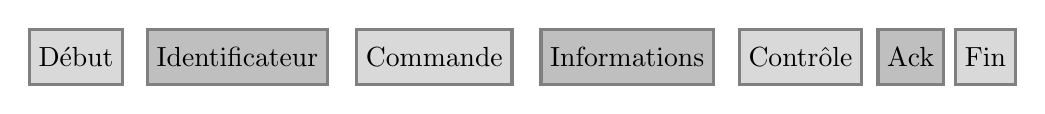
\begin{tikzpicture}[
block1/.style={rectangle, draw=black!50, fill=gray!30, very thick, minimum size=7mm},
block2/.style={rectangle, draw=black!50, fill=gray!50, very thick, minimum size=7mm},
]
%\shorthandoff{:} % Evite le bug de compilation avec tikz
    % Longueurs et espacement
    %\def\longabove{0.2cm}
    \def\espacement{2.35cm}

    % Définition des blocs
    \node [block1] (debut) {Début};
    \node [block2, right of=debut, node distance=2.05cm] (identificateur) {Identificateur};
    \node [block1, right of=identificateur, node distance=2.5cm] (com) {Commande};
    \node [block2, right of=com, node distance=2.45cm] (informations) {  Informations  };
    \node [block1, right of=informations, node distance=2.2cm] (controle) {Contrôle};
    \node [block2, right of=controle, node distance=1.4cm] (ack) {Ack};
    \node [block1, right of=ack, node distance=0.95cm] (fin) {Fin};
 
    % Définition des liens
%    \draw [<-] (codeur) -- ++(-2,0) node[left] {$\{b_n\}$};
%    \draw [->] (codeur) -- node[above=\longabove] {$\{d_n\}$} (cbs);
%    \draw [->] (cbs) -- node[above=\longabove] {$\{c_k\}$} (modulateur);
%    \draw [->] (modulateur) -- ++(2,0) node[right] {$s(t)$};
\end{tikzpicture}

  \caption{Structure de la trame d'un bus de communication CAN.}
  \label{fig:structure-de-trame-blocs}
\end{figure}


Principe de fonctionnement du bus : Structure de trame
Il existe plusieurs format de trames :
- trame de données (data frame)
- trame de requête (remote frame)
- trame de gestion d’erreur (error frame)
- Trame de surcharge (overload frame)
- espace entre trame (inter-frame space)








